\chapter{People detection}
\label{chp:people_detection}
% Explain:
% - Why this is needed
% - How it is implemented
% - Rx beamforming
% - How it works, maybe some points on the accuracy and how it performs on different types of persons

The first step in dynamic multiple people vital signs estimation, is detecting and tracking persons in range of the sensor. In this chapter, the algorithm to detect persons is explained.

\section{Overview}
% Explain what people detection solves
This chapter goes into more detail about detecting people using the radar data. But why is it needed to detect persons in the first place? Every time a measurement has been taken, this measurement consists of the whole field of view of the radar sensor. Apart from the reflections which bounce back from the people in range of the sensor, there are also other reflections, like reflections from static objects like walls, plants and other pieces of furniture in the room. The aim of this chapter is to isolate the persons in the radar data from all of the other data. Then the exact location from the persons is established inside of the radar data, this location can then be used in Chapter~\ref{chp:measuring_vital_signs}, where the actual vital signs estimation is explained.

\section{People detection algorithm}
For this people detection algorithm to work, a heatmap generated from the radar data is needed. This heatmap is a 2 dimensional array of bins. A bin is a 2D area in front of the sensor for which the signal strength is measured. The value in each bin denotes the amount of energy reflected in that location. If there is a high amount of energy that gets reflected back to the sensor, there is a high probability of an object present at that location. 

The goal of this project is vital signs estimation on multiple people. Because this technology is in very early stages of development, it was opted to have a very low noise environment for the radar data gathering. Static noise will be filtered out, this will be explained in Section~\ref{sec:people_detection_implementation}. So apart from the persons present in the view of the sensor, there will be no other sources of reflection present. This means that a fairly basic peak detection algorithm would suffice for this implementation. First, all of the peaks in the heatmap are found, then the peaks close to each other are grouped together. When these processing steps are done, each detected peak is the center location of a person present in the field of view of the radar sensor. See also Figure~\ref{fig:people_detection_block_diagram} for a block diagram of this person detection algorithm.

\begin{figure}[t]
\centering
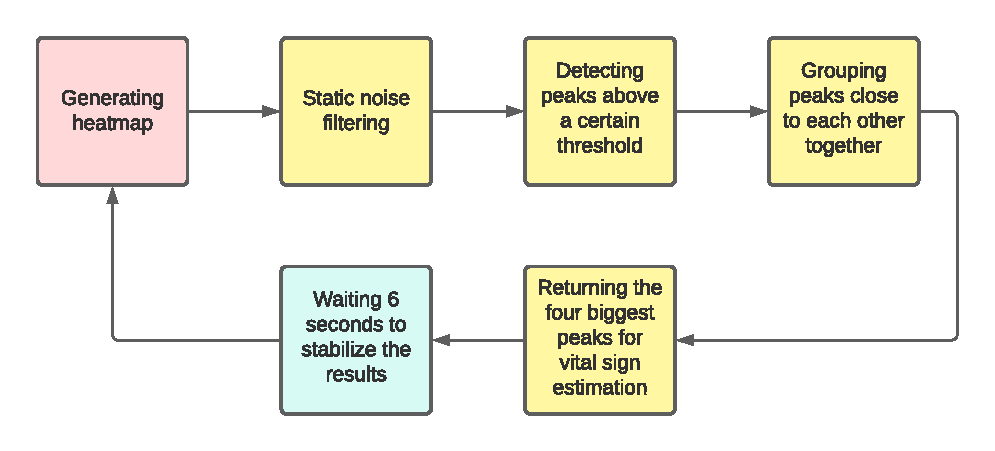
\includegraphics[width=.9\textwidth]{figures/people_detection/People detection algorithm.pdf}
\caption{Block diagram of the processing steps involved in the people detection algorithm.}
\label{fig:people_detection_block_diagram}
\end{figure}

\section{Existing solutions}
There are existing algorithms to group together multiple points with high energy which are close to each other. These groups of points could be an object, a person or any other thing in the space which reflects the RF waves from the sensor. One example is a Constant False Alarm Rate (CFAR) algorithm. This algorithm is already implemented in the mmWave SDK of Texas Instruments \cite{mmwavesdk_website}. This is a very difficult algorithm to set up however, it requires intricate knowledge about the inner workings of the algorithm and of all of the right data streams in the chip. Documentation on how to implement this algorithm was missing, only a working general version is provided. Because of these reasons, a detection algorithm was build from scratch. Because it was build from the ground up, it was ensured that all of the needs and output formats could be met.
% \todo{Add more figures and expand above two sections.}

\section{Implementation}
\label{sec:people_detection_implementation}
This section goes into more detail about the actual implementation of the algorithm on the chip. In each subsection, one step of the algorithm is explained. In Listing~\ref{lst:parameters}, the chirp parameters used in this project can be observed. The exact meaning of each parameter can be found in the mmWave SDK \cite{mmwavesdk_website}.

\begin{lstlisting}[label=lst:parameters, caption=Portion of the parameters file which gets send to the IWR6843 to set it up.]
...
profileCfg 0 60 250 10 40 0 0 98 1 64 2200 0 0 40
frameCfg 0 1 168 0 250 1 0
chirpCfg 0 0 0 0 0 0 0 1
chirpCfg 1 1 0 0 0 0 0 4
...
\end{lstlisting}

\subsection{Input data format}
The algorithm returns a list of coordinates with a maximum of 4 persons. It makes use of the build-in range-FFT, doppler-FFT and angle-FFT implementations, described in Section~\ref{sec:range_estimation_background} to Section~\ref{sec:angle_estimation}. Using these methods, a 2 dimensional heatmap can be generated. On the x-axis are all of the bins in the azimuth (angle) direction and on the y-axis are all of the bins in the range direction. So to recap the information found in Section~\ref{sec:background}, the data in the range direction comes from the range-FFT, and the information in the azimuth direction comes from the angle-FFT. Each bin contains information about the energy level in that bin. In other words, how much signal reflection has been observed in that bin location. 

% TODO add in schematic view of heatmap generation

\subsection{Noise removal}
Before persons can be detected, the amount of background noise needs to be removed. Because with less noise, the persons in front of the sensor will stand out more and will be easier to detect. Also, the signal strength will be improved. For this project the testing is done in one location, so it can be assumed that the sensor will be in a static position and there will be no background change. For each new background, a new calibration round needs to be done. During this calibration, the sensor will scan the space in front of it. It is very important that no other persons or objects other than static ones are at that moment in view of the sensor. The sensor will perform 64 scans and take the average of those scans. This noise map will both be saved on the device and returned to the computer via UART. In this way, the computer can send the values along with all of the other parameters when the sensor is restarted, and the calibration round doesn't need to be run again. When the calibration data is in place, it can be used to remove the noise from each new frame that is coming in. This noise algorithm also corrects for whole rows being over saturated. Those rows can be seen clearly in Figure~\ref{fig:no_noise_removal}. The difference between noise correction and no noise correction can be observed in Figure~\ref{fig:noise_vs_no_noise}.

\begin{figure}[t]
\begin{subfigure}{.45\textwidth}
  \centering
  % include first image
  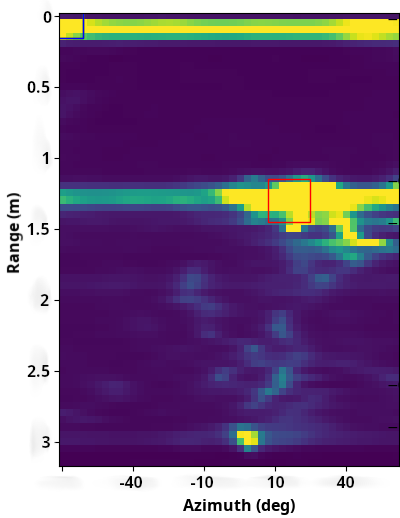
\includegraphics[width=.9\linewidth]{figures/people_detection/heatmap_no_filtering2_crop_axis.png}  
  \caption{Heatmap without any noise removal.}
  \label{fig:no_noise_removal}
\end{subfigure}
\begin{subfigure}{.45\textwidth}
  \centering
  % include second image
  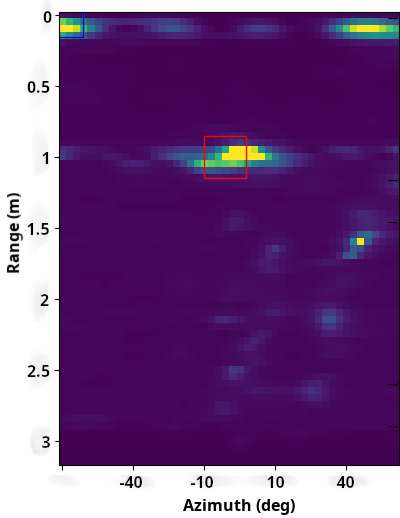
\includegraphics[width=.9\linewidth]{figures/people_detection/heatmap_with_filtering_crop_axis.png}  
  \caption{Heatmap with noise removal implemented.}
  \label{fig:noise_removal}
\end{subfigure}
\caption{These two heatmaps show the difference between noise removal and no noise removal.}
\label{fig:noise_vs_no_noise}
\end{figure}

\subsection{Peak detection}
This algorithm works by detecting peaks. During the testing phase, it was determined what the minimal peak height is for a person in the frame. The maximum heat in one heatmap bin is \texttt{32000}. The minimal peak generated by a person in a frame is \texttt{2000}. These numbers have no unit, it is just a measure for signal strength were \texttt{0} is no signal and \texttt{32000} is the maximum observable signal. This is the first filter, only the peaks which are higher than the threshold are considered.

For this application, it is assumed that each person is sitting approximately half a meter to one meter apart, this makes it easier to detect individual persons. This translates in the grouping functionality of the person detection algorithm. For each new peak that is found, it is checked if there has been another peak found within half a meter of the new peak. If that's the case, the peak with the largest magnitude will be added to the list. This results in finding the biggest peak for each person, provided they sit half a meter apart. The biggest peak gives the information with the highest SNR value, such that the following algorithms will work in the most optimal form. The return value is an array with the coordinates of one or more bins, one bin per person.

This algorithm is executed once every 64 frames. Since the program processes around 10 frames per second, every 6.4 seconds there will be another person detection round performed. The algorithm is not run every frame because it takes relatively much time to compute, and the whole system is more stable in this way. In the future, it would be best to implement a sliding window and take the average of multiple frames to base the tracking on. For this project that could not be implemented, because there was not enough space on the chip and there was no time left for additional calculations. This could be solved by software optimizations.

\begin{algorithm}
\caption{Person finding algorithm}\label{alg:person_finding_algorithm}
\begin{algorithmic}
\Require $heatmap$
\State $maxPeaks \gets list()$
\For{$x=0,1,\ldots,azimuthLength$}
    \For{$y=0,1,\ldots,rangeLength$}
        \State $bin \gets heatmap(x, y)$
        \If{$bin > 2000$}
            \If{$bin$ heat is larger than surrounding bins}
                \If{bin $c$ in $heatmap$ with distance $<$ 0.5 meter}
                    \If{$bin > c$}
                        \State Add $bin$ to $maxPeaks$
                        \State Remove $c$ from $maxPeaks$
                    \EndIf
                \Else
                    \State Add $bin$ to $maxPeaks$
                \EndIf
            \EndIf
        \EndIf
    \EndFor
\EndFor
\end{algorithmic}
\end{algorithm}

\subsection{Result}
In Algorithm~\ref{alg:person_finding_algorithm}, an overview of the algorithm in pseudo code can be found. Figure~\ref{fig:person_detection_two} shows the heatmap result if two persons are sitting in front of the sensor. The red and yellow boxes are drawn exactly in the middle the peak that is detected. These peaks will be used internally for vital signs estimation, this is purely a visualization for the user. In Figure~\ref{fig:person_detection_four}, four persons are detected at the same time. This is possible, but it becomes really crowded in this relatively confined space. The most optimal way for the users will be measuring one or two persons at the same time, which will also become apparent later in this thesis. 

% TODO insert conclusion?

\begin{figure}[t]
\centering
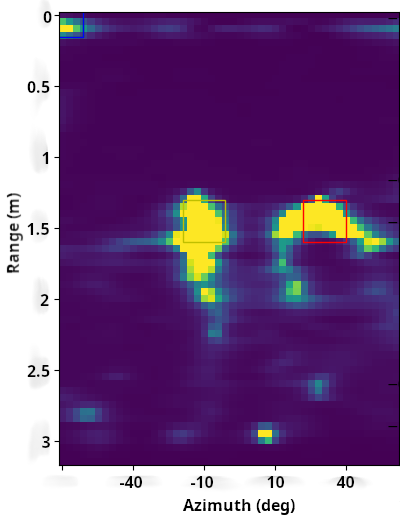
\includegraphics[width=.5\textwidth]{figures/people_detection/multiple_3_crop_axes.png}
\caption{Two persons at the same time detected. Each detected person gets a box drawn around it with a color.}
\label{fig:person_detection_two}
\end{figure}

\begin{figure}[t]
\centering
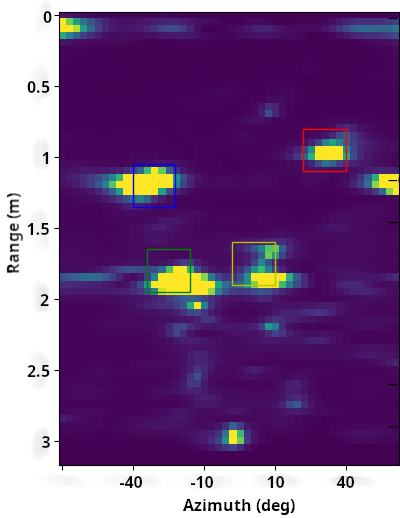
\includegraphics[width=.5\textwidth]{figures/people_detection/4_2_crop_axis.png}
\caption{Four persons at the same time detected. Each detected person gets a box drawn around it with a color.}
\label{fig:person_detection_four}
\end{figure}